\vspace*{\fill}
\begin{center}
    {\color{Black} \rule{\linewidth}{1.2mm} }\\
\vspace{0.25in}
    {\centering\fontsize{30}{40}{\bfseries{\color{Black}{\scshape{Chapter III : Dataset Collection}}}}}
\vspace{0.35in}\\
    {\color{Black} \rule{\linewidth}{1.2mm} }
\end{center}
\vspace*{\fill}
\addcontentsline{toc}{chapter}{\color{Black}{Chapter III : Dataset Collection}}
\setcounter{section}{0}

\newpage

\section{Introduction}
\hspace{\parindent}
In this chapter we will try to find the best dataset that will help us with our problem, by performing a comparison between all the available datasets and their annotations, we can see that there is a lot of datasets which are created to attack a specific sets of problems, we can see below all available datasets:

\section{ALL-IDB}
\hspace{\parindent}
ALL-IDB (Acute Lymphoblastic Leukemia Image Database for Image Processing) \textsuperscript{\cite{labati2011all}} is a public and free dataset, specifically designed for the evaluation and the comparison of algorithms for segmentation and image classification. The database focus on Acute Lymphoblastic Leukemia (ALL), Acute is a type of blood cancer that starts in white blood cells in bone marrow, the soft inner part of bones. It develops from immature lymphocytes, a kind of white blood cell that’s key to immune system.\textsuperscript{\cite{Annie_Stuart_What_2022_webmd}}.\

Each image in the dataset, Contains classification/position of ALL lymphoblasts is provided by expert oncologists. A lymphoblast is a modified naive lymphocyte with altered cell morphology. It occurs when the lymphocyte is activated by an antigen.\

The images of the dataset has been captured with an optical laboratory microscope coupled with a Canon PowerShot G5 camera. All images are in JPG format with 24 bit color depth, resolution 2592 x 1944. the ALL-IDB divides on two Datasets ALL-IDB1 and ALL-IDB2.\

\subsection{Dataset ALL-IDB1}
\hspace{\parindent}
The ALL-IDB1 can be used for segmentation or classification with image processing methods or Artificial intelligence models. The dataset is composed of 108 images collected during September, 2005. It contains about 39000 blood elements, where the lymphocytes has been labeled by expert oncologists.

\begin{figure}[H]
\centering
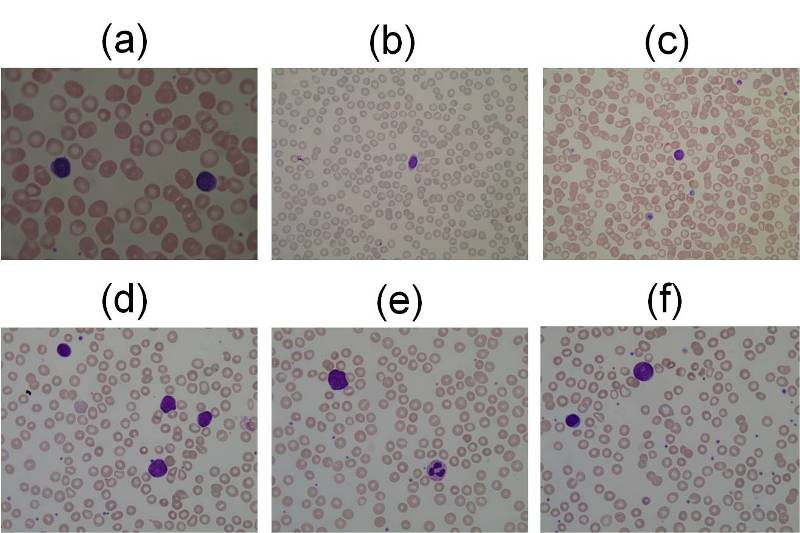
\includegraphics[width = 5in, height = 3in]{../images/ALLIDB1.jpg}
\caption{Examples of the images contained in ALL-IDB1: healthy cells from non-ALL patients (a,b,c), probable lymphoblasts from ALL patients (d,e,f). }
\end{figure}

\textbf{annotation:} input image ''Im006\_1.jpg'' (a) and the related classification file ''Im006\_1.xyc'' reporting the coordinates of the centroids of probable ALL lymphoblasts (b).

\begin{figure}[H]
\begin{minipage}[b]{0.35\linewidth}
\centering
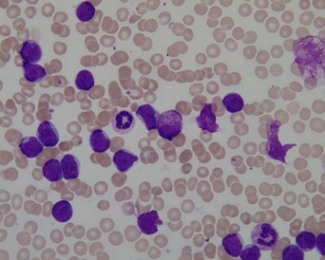
\includegraphics{../images/Im006_1.jpg}
\subcaption{Im006\_1.jpg}
\label{fig:Im006.jpg}
\end{minipage}
\hfill
\begin{minipage}[b]{0.3\linewidth}
\centering
\lstinputlisting[breaklines]{../images/Im006\_1.xyc}
\subcaption{Im006\_1.xyc}
\label{fig:Im006.xyc}
\end{minipage}

\begin{minipage}[b]{0.35\linewidth}
\centering
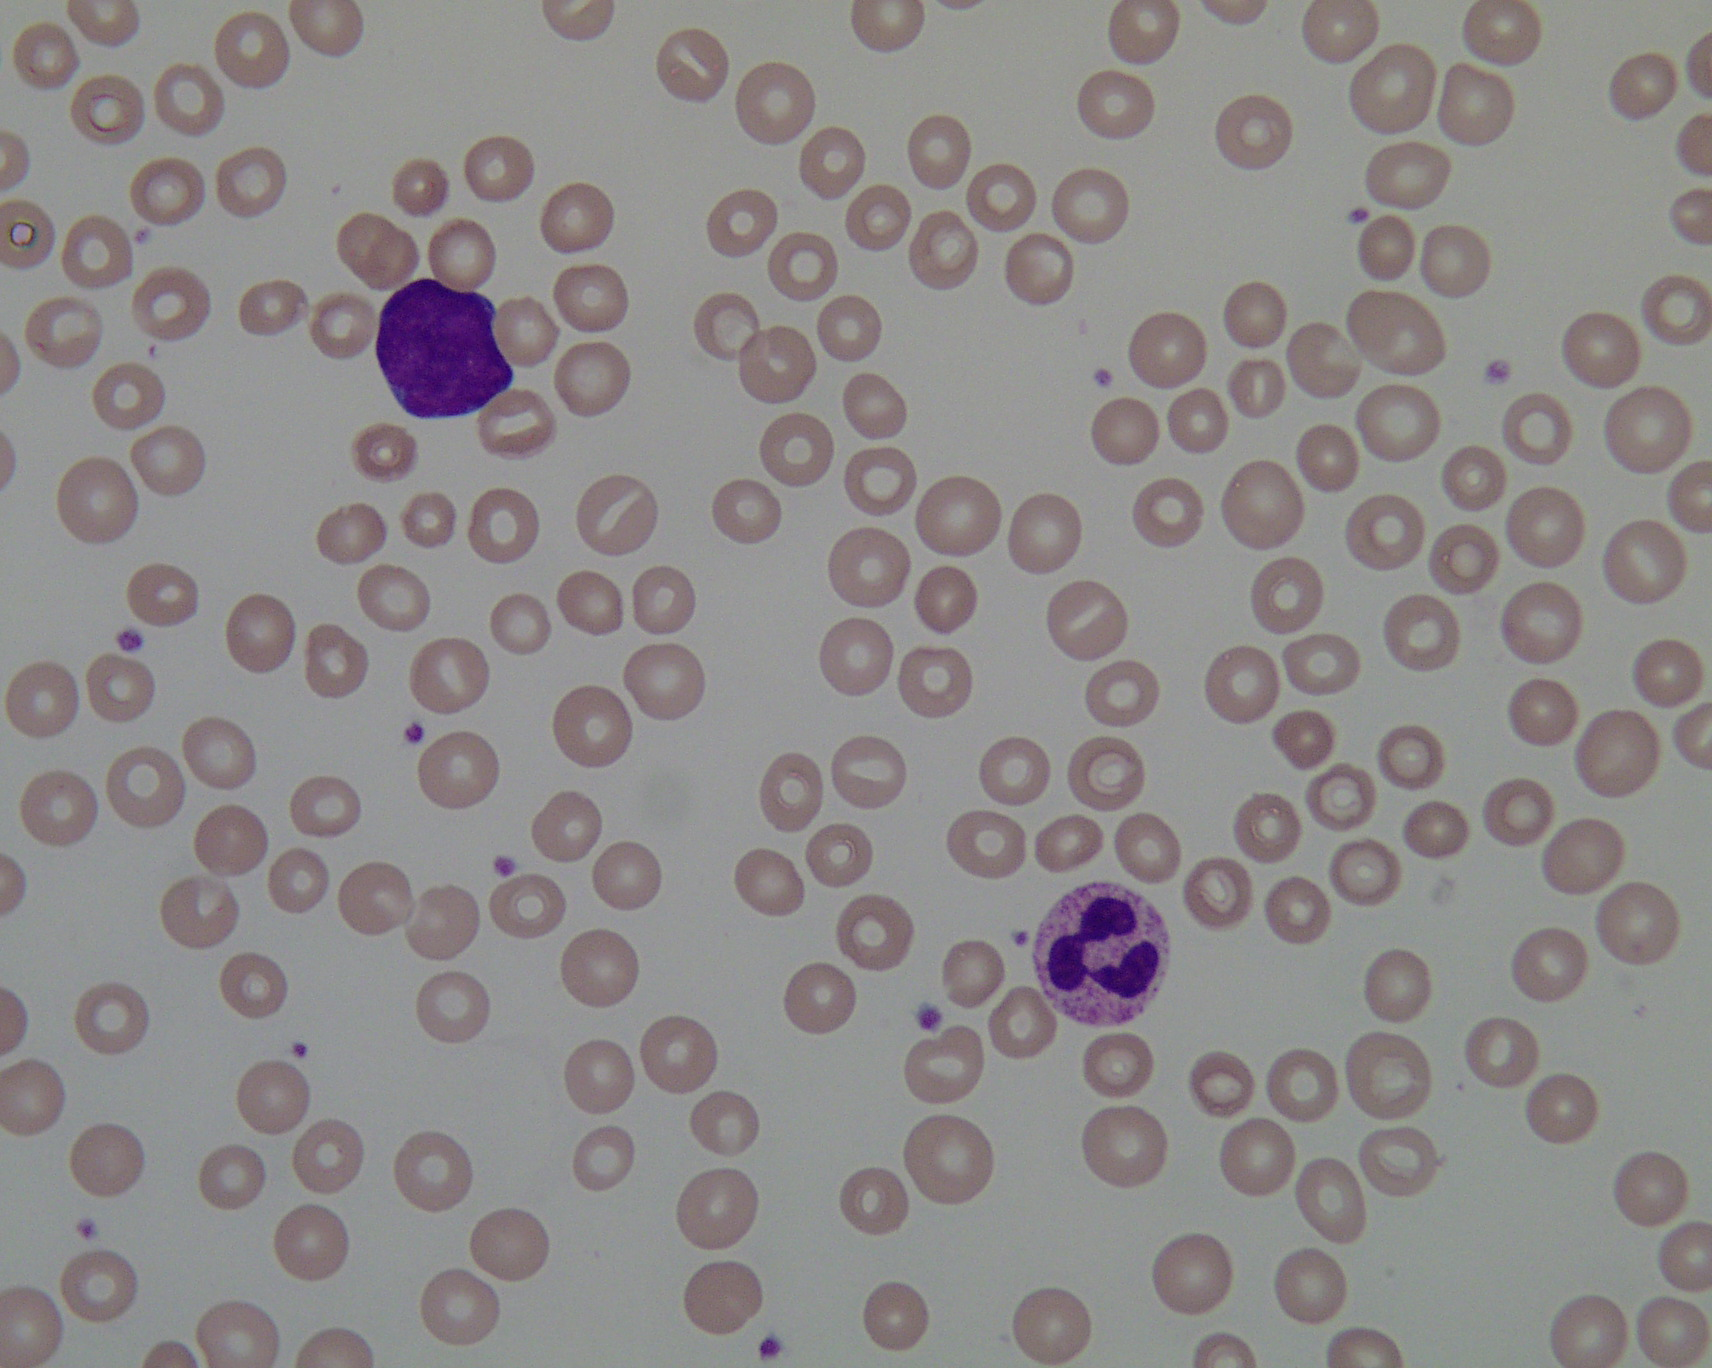
\includegraphics[width=57mm]{../images/Im033_1.jpg}
\subcaption{Im033\_1.jpg}
\label{fig:Im033.jpg}
\end{minipage}
\hfill
\begin{minipage}[b]{0.3\linewidth}
\centering
\lstinputlisting[breaklines]{../images/Im033\_1.xyc}
\subcaption{Im033\_1.xyc}
\label{fig:Im033.xyc}
\end{minipage}
\caption{Sample data from the ALL-IDB1 Database}
\end{figure}

The ALL-IDB1 image files are named with the notation ImXXX\_Y.jpg where XXX is a 3-digit integer counter and Y is a boolean digit equal to 0 if no blast cells are present, and equal to 1 if at least one blast cell is present in the image. All images labeled with Y=0 are from for healthy individuals, and all images labeled with Y=1 are from ALL patients. Each image file ImXXX\_Y.jpg (figure \ref{fig:Im006.jpg}, \ref{fig:Im033.jpg}) is associated with a text file ImXXX\_Y.xyc (figure \ref{fig:Im006.xyc}, \ref{fig:Im033.xyc}) reporting the coordinates of the centroids of the blast cells, if any.\\

If we plot the coordinates in the Img006\_1.xyc (figure \ref{fig:Im006.jpg}) file on the image Im006\_1.jpg (figure \ref{fig:Im006.xyc}) we get the figure \ref{fig:Im006.xyc.jpg}

\newpage

\begin{figure}[H]
\centering
    \fbox{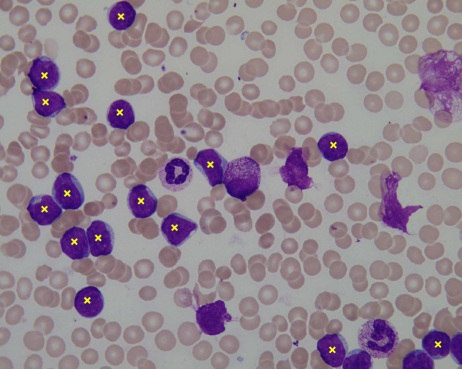
\includegraphics[width = 5in, height = 4in]{../images/img006.xyc.jpg}}
\caption{coordinates from Img006\_1.xyc plotted on Img006\_1.jpg}
\label{fig:Im006.xyc.jpg}
\end{figure}

\subsection{Dataset ALL-IDB1}
\hspace{\parindent}
This dataset has been created for testing the performances of classification systems. where the dataset has no segmentation information it contains only one information which is the presence of ALL lymphoblasts, the dataset is a collection of cropped area of interest of normal and blast cells that belongs to the ALL-IDB1 dataset as we can see in figure \ref{fig:ALL-IDB2}

\begin{figure}[H]
\centering
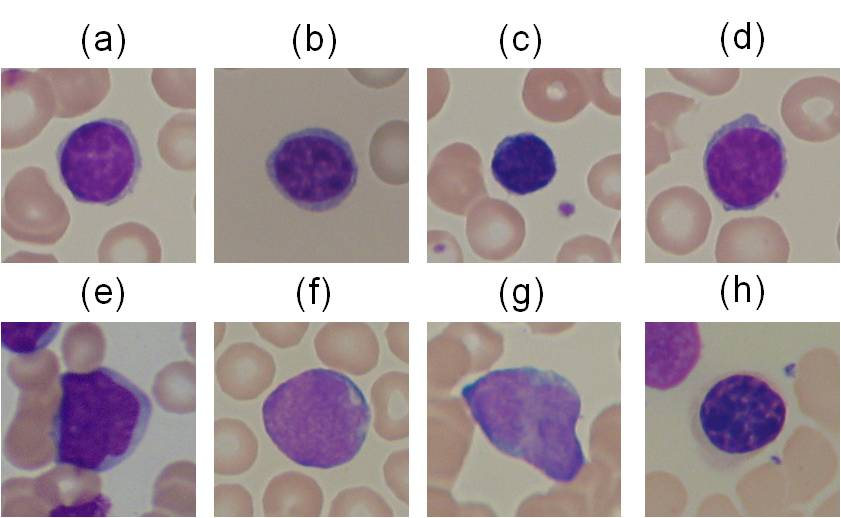
\includegraphics{../images/ALL-IDB2.jpg}
\caption{Examples of the images contained in ALL-IDB2: healthy cells from non-ALL patients (a-d), probable lymphoblasts from ALL patients (e-h).}
\label{fig:ALL-IDB2}
\end{figure}

\vspace{-0.14in}

The annotation of ALL-IDB2 is similar to the ALL-IDB1 but with no centroid coordinates. The ALL-IDB2 image files are named with the notation ImXXX\_Y.jpg where XXX is a progressive 3-digit integer and Y is a Boolean digit equal to 0 if the cell placed in the center of the image is not a blast cell, and equal to 1 if the cell placed in the center of the image is a blast cell. all images labeled with Y=0 are from for healthy individuals, and all images labeled with Y=1 are from ALL patients. 

\section{Broad Bio-image Benchmark Collection}
\hspace{\parindent}
The Broad Bio-image Benchmark Collection (BBBC) is a collection of freely downloadable microscopy image sets, cited in 450+ studies. In addition to the images themselves, each set includes a description of the biological application and some type of "ground truth" (expected results) \textsuperscript{\cite{ljosa2012annotated}}. The BBBC is organized by the Broad Institute's Imaging Platform.\

The dataset contains 54 image collections of various cell types, each collection has at least one of 6 ground truth types such as cell count, foreground / background, outlines of objects, biological labels, location and bounding boxes. in the sections below we describe each ground truth:

\subsection{Cell counts}
\hspace{\parindent}
In this case, the ground truth consists of the number of cells (or other objects) in each image, as counted by one or more humans. for example in BBBC1(Human HT29 colon-cancer cells) we have an image in figure \ref{fig:BBBC1} with the labels file in figure \ref{fig:BBBC001_Counts}:

\begin{figure}[H]
\begin{minipage}[c]{\linewidth}
\centering
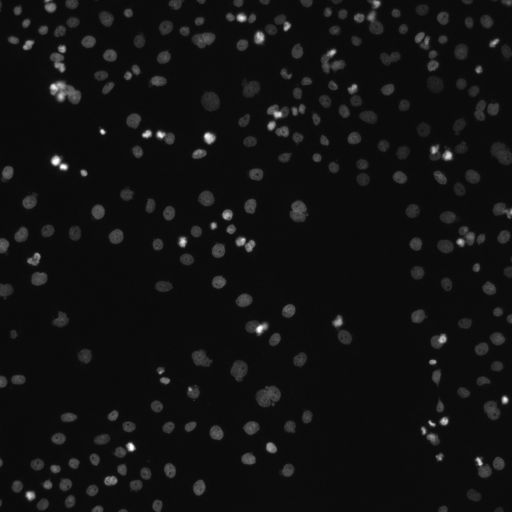
\includegraphics[width = 2.5in, height = 1.8in]{../images/AS_09125_050118150001_A03f05d0.jpg}
\subcaption{AS\_09125\_050118150001\_A03f05d0.jpg}
\label{fig:BBBC1}
\end{minipage}

\begin{minipage}[c]{\linewidth}
\centering
\lstinputlisting[breaklines]{../images/BBBC001_v1_counts.txt}
\subcaption{BBBC001\_v1\_counts.txt}
\label{fig:BBBC001_Counts}
\end{minipage}
\caption{Sample data from the BBBC1 Database with counts Ground truth}
\end{figure}

in the figure \ref{fig:BBBC001_Counts} we can see the two counts performed by two experts, for the image \ref{fig:BBBC1} the first expert have found 241 cells but the second one found 257 cells.

\subsection{Foreground and background}
\hspace{\parindent}
In this case, a human produces a binary (black and white but in some cases thy use other colors) image the same size as the original image. Pixels that belong to the foreground (i.e., the cells or other objects) are white, and pixels that belong to the background are black. in the example below (figure \ref{fig:BBBC004_img} and \ref{fig:BBBC004_F}) we can see the image and the corresponding mask where the cells colored with blue and the background with black.

\begin{figure}[H]
\begin{minipage}[c]{0.4\linewidth}
\centering
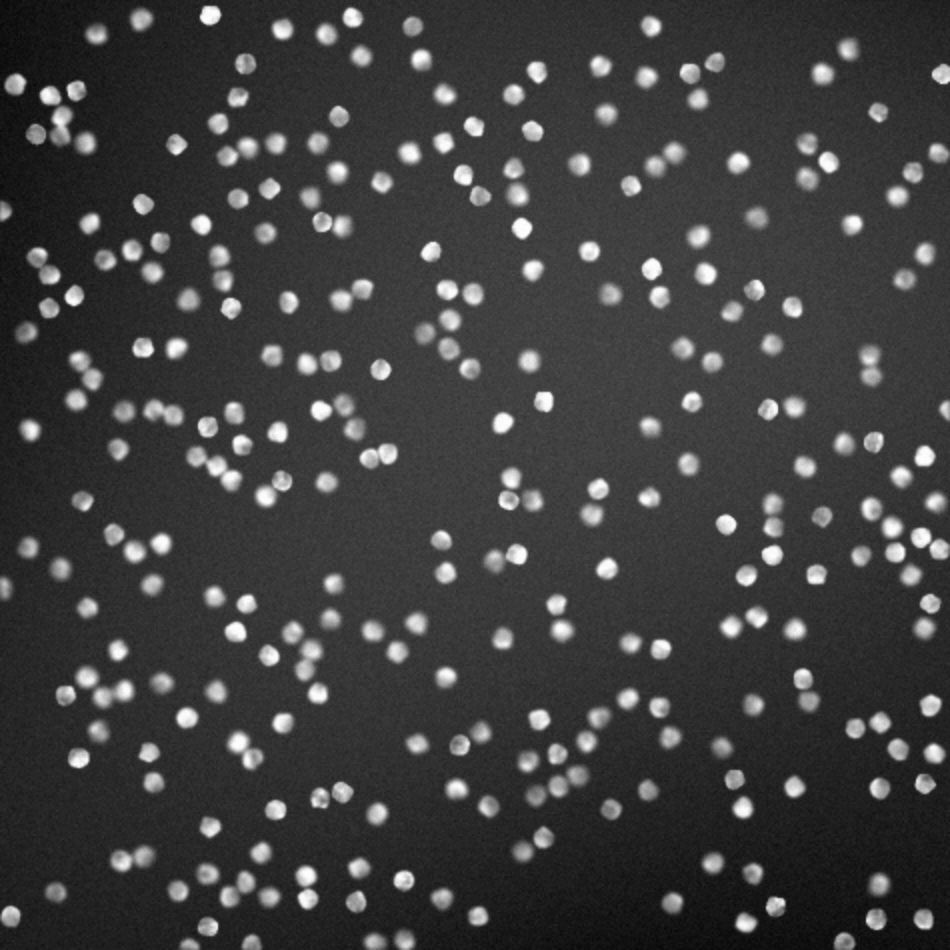
\includegraphics[width=70mm]{../images/BBBC4-1.jpg}
\subcaption{2Gray1.tif (image)}
\label{fig:BBBC004_img}
\end{minipage}
\hfill
\begin{minipage}[c]{0.4\linewidth}
\centering
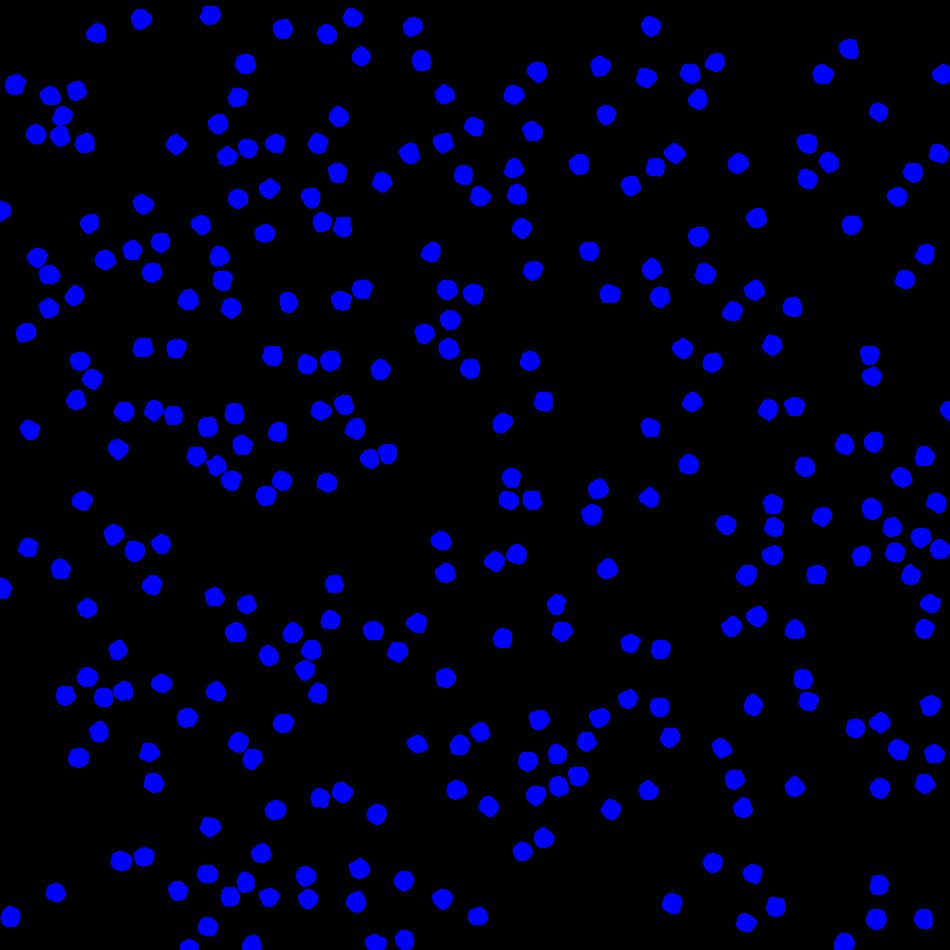
\includegraphics[width=70mm]{../images/BBBC4-1-F.jpg}
\subcaption{1.tif (mask)}
\label{fig:BBBC004_F}
\end{minipage}
\caption{Sample data from the BBBC4 Database with mask as ground truth}
\end{figure}

\subsection{Outlines of individual objects}
\hspace{\parindent}
In this case, a human outlines each cell in the image in order to indicate which pixels belong to which cell. The ground truth is provided as binary images, with black outlines on a white background.

\begin{figure}[H]
\begin{minipage}[c]{0.4\linewidth}
\centering
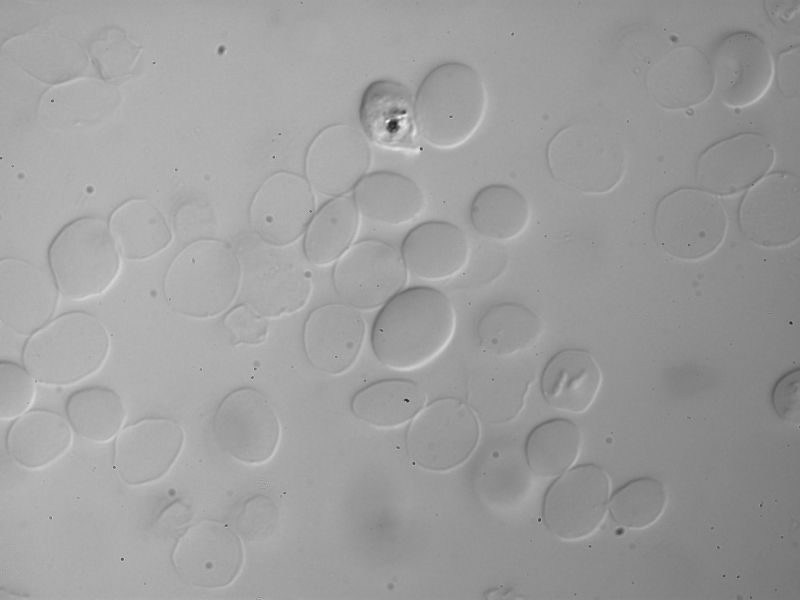
\includegraphics[width=70mm]{../images/48hr-001-DIC.jpg}
\subcaption{48hr-001-DIC.jpg (image)}
\label{fig:BBBC009_img}
\end{minipage}
\hfill
\begin{minipage}[c]{0.4\linewidth}
\centering
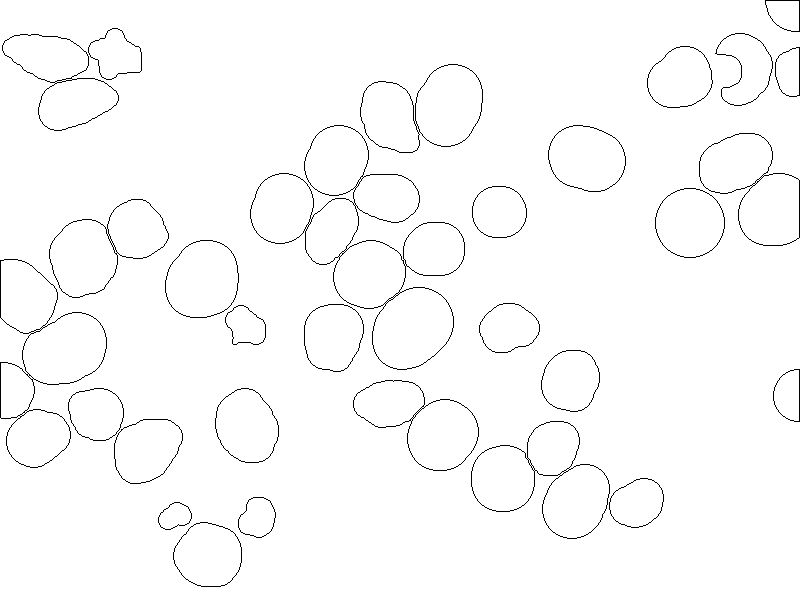
\includegraphics[width=70mm]{../images/48hr-001-DIC_.jpg}
\subcaption{48hr-001-DIC.jpg (edge mask)}
\label{fig:BBBC009_O}
\end{minipage}
\caption{Sample data from the BBBC9 Database with edge mask (outlines) as ground truth}
\end{figure}

\subsection{Biological labels}
\hspace{\parindent}
In these cases, the experiments have been prepared with control samples for which we know the expected biological result. The types of controls that are available dictate the type of statistic that can be calculated.

\subsection{Location}
\hspace{\parindent}
In this case, the ground truth consists of the X, Y, and optionally Z location of objects (typically their centroids similar to ALL-IDB1 Annotation \ref{fig:Im006.xyc.jpg}) .

\subsection{Bounding Boxes}
\hspace{\parindent}
Bounding boxes are rectangles completely enclosing an object.

\vspace{-0.1in}

\section{WBC Image Dataset : Fast and Robust Segmentation of White Blood Cell Images by Self-supervised Learning}
\hspace{\parindent}
This is two datasets of white blood cell (WBC) images used for “Fast and Robust Segmentation of White Blood Cell Images by Self-supervised Learning”, which can be used to evaluate cell image segmentation methods \textsuperscript{\cite{Zheng2018}}.\
This collection contains two datasets different from each other in terms of the image color, cell shape, background, etc. The ground truth segmentation results are manually sketched by domain experts, where the nuclei, cytoplasms and background including red blood cells are marked in white, gray and black respectively. 

\subsection{Dataset 1}
\hspace{\parindent}
Was obtained from Jiangxi Tecom Science Corporation \textsuperscript{\cite{2022_tecom-cn}}, China. It contains three hundred 120×120 images of WBCs and their color depth is 24 bits. The images were taken by a Motic Moticam Pro 252A optical microscope camera with a N800-D motorized auto-focus microscope.

\begin{figure}[H]
\centering
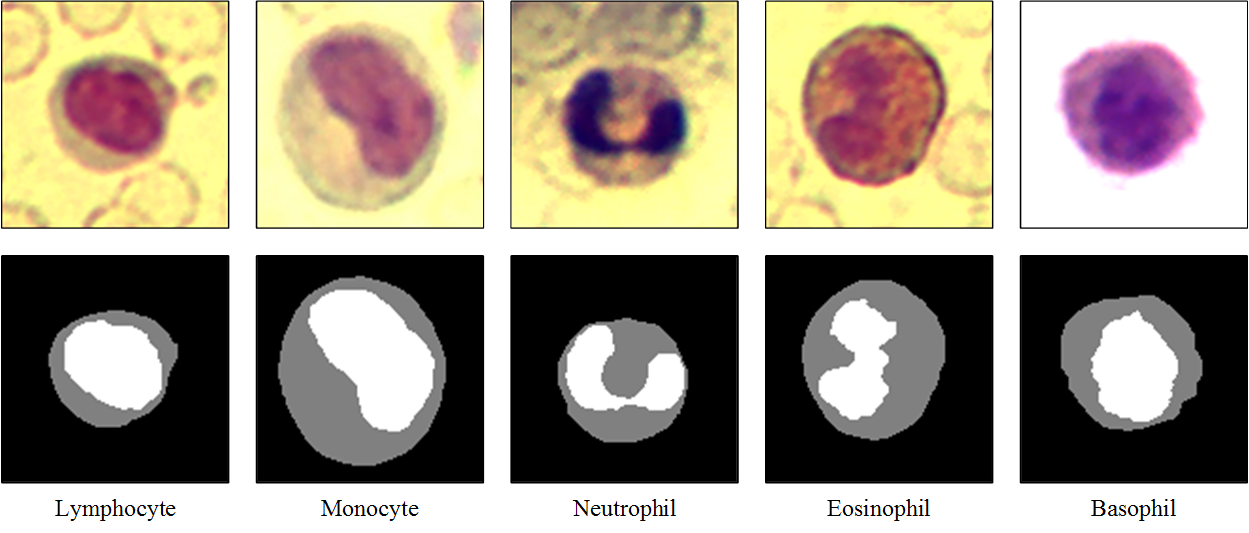
\includegraphics[width=5.2in]{../images/WBC_Dataset1.png}
\caption{Sample data from WBC\_Segmentaion Dataset 1}
\label{fig:WBC_Dataset1_sample}
\end{figure}

\subsection{Dataset 2}
Consists of one hundred 300×300 color images, which were collected from the Cella-Vision blog \textsuperscript{\cite{2022_cellavision}}. The cell images are generally purple and may contain many red blood cells around the white blood cells.

\begin{figure}[H]
\centering
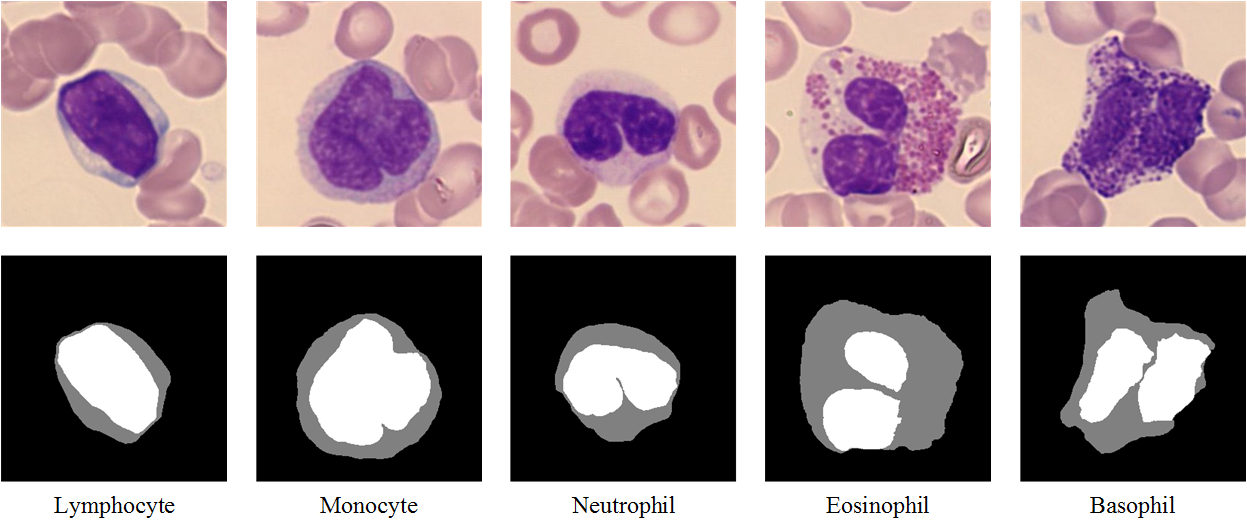
\includegraphics[width=5.2in]{../images/WBC_Dataset2.png}
\caption{Sample data from WBC\_Segmentaion Dataset 2}
\label{fig:WBC_Dataset2_sample}
\end{figure}

\subsection{Annotation}
\hspace{\parindent}
The class labels of each image in Dataset 1 and Dataset 2 are stored in csv files. The labels (1- 5) represent neutrophil, lymphocyte, monocyte, eosinophil and basophil, respectively.


\subsection{A large dataset of white blood cells containing cell locations and types, along with segmented nuclei and cytoplasm}
\hspace{\parindent}
The database is provided by \href{https://raabindata.com/free-data/#double-labeled-cropped-cells}{RabinData} and \textsuperscript{\cite{Kouzehkanan2022}} which divides on two separate datasets:

\subsubsection{Raabin-WBC Data}
\hspace{\parindent}
Contains 4 sub-Datasets:
\begin{itemize}
    \item \textbf{Double-labeled cropped cells} : Double-labeled cropped cells are also provided containing only five main classes including mature neutrophils, lymphocytes (small and large), eosinophils, monocytes, and basophils. 
    \item \textbf{Nucleus\_cytoplasm\_Ground truths} : in this sub-Dataset they prepared the ground truths of the cytoplasm and the nucleus for a proper number of cropped white blood cells. For this purpose, 1145 cropped images including 242 lymphocytes, 242 monocytes, 242 neutrophils, 201 eosinophils, and 218 basophils were randomly selected, and their ground truths were extracted by an expert.
    \item \textbf{Microscopic images were taken by the Olympus CX18 microscope and the Samsung Galaxy S5 camera and the 4th database with contain images taken by Zeiss microscope and the LG G3 camera } : in these two sub-Datasets. Corresponding to each microscopic image, a dictionary (json format) file containing the following information about that image was provided:
    \begin{itemize}
        \item Information about the blood elements in the image including their coordinates and labels.
        \item Information about the blood smears including staining method and the type of the disease.
        \item Information about the microscope includes the type of microscope and its magnification size.
        \item The type of camera used.
    \end{itemize}
\end{itemize}

\subsubsection{Raabin-Leukemia Data}
\hspace{\parindent}
Contains 4 sub-Datasets:
\begin{itemize}
    \item \textbf{Acute Lymphoblastic Leukemia}  
    \item \textbf{Acute Myeloblastic Leukemia} 
    \item \textbf{Chronic Lymphocytic Leukemia}
    \item \textbf{Chronic Myelogenous Leukemia}
\end{itemize}
In each of these sub-Dataset, All samples were taken from patients who had referred to our collaborator medical laboratory (Takht-e Tavous Laboratory in Tehran, Iran). It should be notices Zeiss microscope and LG J3 smartphone camera had been used for imaging.

\subsection{BCCD}
\hspace{\parindent}
BCCD (Blood Cell Count and Detection) Dataset is a small-scale dataset for blood cells detection. The dataset contains a total of 364 (640x480) jpeg images with their annotations. The original data and annotations are from \href{https://github.com/cosmicad/dataset}{cosmicad} and \href{https://github.com/akshaylamba/all_CELL_data}{akshaylamba}.\\
In this project, the Faster R-CNN algorithm from keras-frcnn for Object Detection is used. From this dataset, nicolaschen1 developed two Python scripts to make preparation data (CSV file and images) for recognition of abnormalities in blood cells on medical images.

\begin{figure}[H]
\centering
    \fbox{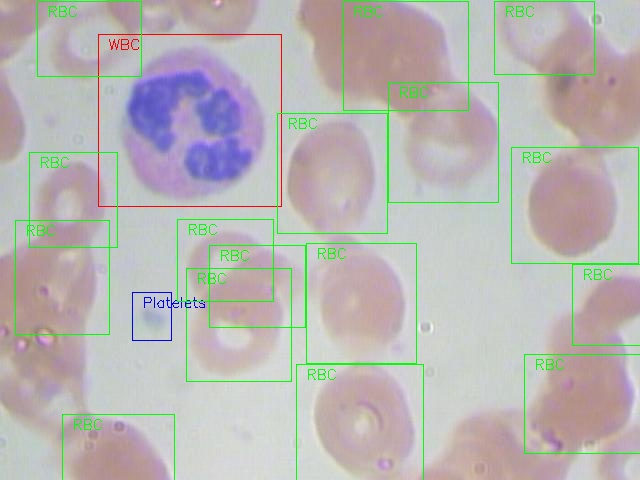
\includegraphics[width = 4.2in, height = 3.5in]{../images/BBCD1.jpg}}
\caption{Sample data from BBCD}
\label{fig:BBCD1}
\end{figure}

In this database they use bounding boxes to locate the cells and each bounding box has the type of cell RBC or WBC and Platelets. they are using the VOC format as a database architecture.

\section{Dataset resume}
\hspace{\parindent}

\begin{table}[H]
\centering
\resizebox{\textwidth}{!}{%
\begin{tabular}{|c|c|ccc|c|c|}
\hline
\cellcolor[HTML]{FFFFFF}\textbf{\begin{tabular}[c]{@{}c@{}}Dataset\\ Name\end{tabular}} &
  \cellcolor[HTML]{FFFFFF}\textbf{\begin{tabular}[c]{@{}c@{}}Dataset\\ Size\end{tabular}} &
  \multicolumn{3}{c|}{\textbf{\begin{tabular}[c]{@{}c@{}}Type of cells\\ (RBC, WBC, Platelets)\end{tabular}}} &
  \cellcolor[HTML]{FFFFFF}\textbf{Type of annotation} &
  \cellcolor[HTML]{FFFFFF}\textbf{Description} \\ \hline
\cellcolor[HTML]{FFFFFF}ALL-IDB \textsuperscript{\cite{pm77-2n23-20}}&
  \cellcolor[HTML]{FFFFFF}108 &
  \multicolumn{1}{c|}{108 masks / 13 edges} &
  \multicolumn{1}{c|}{108 masks} &
  108 masks&
  \cellcolor[HTML]{FFFFFF}\begin{tabular}[c]{@{}c@{}}Location \\ (Centroid of cells)\end{tabular} &
  \cellcolor[HTML]{FFFFFF}\begin{tabular}[c]{@{}c@{}}Acute Lymphoblastic\\ Leukemia Image Database\\ for Image Processing\end{tabular} \\ \hline
\cellcolor[HTML]{FFFFFF}BBBC \textsuperscript{\cite{ljosa2012annotated}} &
  \cellcolor[HTML]{FFFFFF}Lots of subdatasets &
  \multicolumn{1}{c|}{X} &
  \multicolumn{1}{c|}{X} &
  X &
  \cellcolor[HTML]{FFFFFF}\begin{tabular}[c]{@{}c@{}}All types of\\ annotations\end{tabular} &
  \cellcolor[HTML]{FFFFFF}\begin{tabular}[c]{@{}c@{}}Broad Bioimage Benchmark\\ Collection\end{tabular} \\ \hline
\cellcolor[HTML]{FFFFFF}WBC Image Dataset &
  \cellcolor[HTML]{FFFFFF}400 &
  \multicolumn{1}{c|}{} &
  \multicolumn{1}{c|}{X} &
   &
  \cellcolor[HTML]{FFFFFF}\begin{tabular}[c]{@{}c@{}}Foreground and\\ Background (mask)\end{tabular} &
  \cellcolor[HTML]{FFFFFF}\begin{tabular}[c]{@{}c@{}}WBC Image Dataset : \\ Fast and Robust Segmentation\\ of White Blood Cell Images\\ by Self-supervized Learning\end{tabular} \\ \hline
    BCCD \textsuperscript{\cite{BCCD_Dataset}} &
  364 &
  \multicolumn{1}{c|}{} &
  \multicolumn{1}{c|}{x} &
   &
  Bounding boxes &
  Blood Cell Count and Detection \\ \hline
\end{tabular}%
}
\caption{Table that resumes datasets mentioned above}
\label{Table that resumes datasets mentioned above}
\end{table}


\section{Conclusion}
\hspace{\parindent}
In this chapter we explored all the available datasets and their annotations which can help us in our problem, we decided to work with the updated ALL-IDB1 dataset which has 13 RBC edges and masks, 108 WBC, Platelets Masks and 13 RBC images which has the count information, but the WBC and Platelets donthave the count information where we had to use manual count and algorithms to find the count information for these images.

\newpage
